\documentclass[10pt]{article}
\usepackage[ngerman]{babel}
\usepackage[utf8]{inputenc}
\usepackage[T1]{fontenc}
\usepackage{graphicx}
\usepackage[export]{adjustbox}
\graphicspath{ {./images/} }
\usepackage{amsmath}
\usepackage{amsfonts}
\usepackage{amssymb}
\usepackage[version=4]{mhchem}
\usepackage{stmaryrd}
\usepackage{hyperref}
\hypersetup{colorlinks=true, linkcolor=blue, filecolor=magenta, urlcolor=cyan,}
\urlstyle{same}
\usepackage{multirow}

\title{Gstudocu }

\author{}
\date{}


\begin{document}
\maketitle
\section*{WBE Zusammenfassung}
\begin{center}

\includegraphics[width=\linewidth]{images/2024_12_29_858f09cde51177c71657g-01}
\end{center}

Scanne, um auf Studocu zu öffnen

\section*{Zusammenfassung - WBE}
\section*{Contents}
JavaScript. ..... 4\\
Grundlagen ..... 4\\
Web-Konsole ..... 4\\
Datentypen ..... 4\\
Vergleich mit $==$ oder $==$ ..... 4\\
Variablenbindung ..... 4\\
Verzweigungen, Wiederholung, switch case. ..... 5\\
Funktionsdefinition ..... 5\\
Objekte und Arrays. ..... 5\\
Objekte ..... 5\\
Json (JavaScript Object Notation) ..... 7\\
Funktionen. .....  8\\
Modulsystem in JavaScript. .....  8\\
Prototypen von Objekten .....  8\\
Call, apply, bind .....  9\\
Klassen ..... 9\\
Vererbung. .....  9\\
Getter und Setter ..... 10\\
Asynchrones Programmieren ..... 10\\
File API ..... 10\\
Callbacks ..... 11\\
SetTimeout ..... 11\\
SetInterval ..... 11\\
SetImmediate ..... 12\\
Event-Modul (EventMitter) ..... 12\\
Promises ..... 12\\
Webserver ..... 15\\
Server im Internet ..... 15\\
File-Transfer (File Server) ..... 15\\
HTTP ..... 15\\
Node.js Webserver ..... 16\\
REST API ..... 17\\
Express.js ..... 17\\
Jasmine (Testing) ..... 18\\
Browser-Technologien ..... 20\\
Vordefinierte Objekte ..... 20\\
document ..... 20\\
window ..... 20\\
navigator. ..... 20\\
location ..... 20\\
Document Object Model ..... 21\\
Element auffinden ..... 21\\
Textknoten erzeugen ..... 21\\
Elementknoten erzeugen ..... 21\\
Attribut setzen ..... 22\\
Style anpassen ..... 22\\
Event handling ..... 23\\
Event abonnieren/entfernen ..... 23\\
Tastatur-Events ..... 23\\
Mauszeiger-Events ..... 24\\
Scroll-Events ..... 24\\
Fokus- und Ladeereignisse ..... 24\\
Jquery ..... 25\\
Web-Grafiken ..... 26\\
SVG ..... 26\\
Canvas ..... 26\\
Browser-API ..... 27\\
Web Storage ..... 27\\
Local Storage ..... 27\\
History ..... 27\\
GeoLocation ..... 27\\
Formulare ..... 28\\
Formular Events ..... 29\\
GET/POST-Methode ..... 29\\
Cookies und Sessions ..... 30\\
Cookies ..... 30\\
Sessions ..... 30\\
Fetch API ..... 31\\
Response Objekt ..... 31\\
UI-Bibliothek ..... 32\\
Dom-Scripting und Abstraktionen ..... 32\\
JSX und SJDON ..... 32\\
SuiWeb ..... 32

\section*{JavaScript}
\section*{Grundlagen}
\section*{Web-Konsole}
In JavaScript kann man die Web-Konsole ganz einfach mit dem Keyword «console» ansprechen.

\begin{center}
\begin{tabular}{|l|l|}
\hline
console.log(message) & Meldung in der Konsole loggen \\
\hline
console.clear() & Konsole löschen \\
\hline
console.trace(message) & Stack trace ausgeben \\
\hline
console.time() & Timer starten \\
\hline
console.timeEnd() & Timer stoppen \\
\hline
console.error(message) & stderr ausgeben \\
\hline
\end{tabular}
\end{center}

Webseite für Konsolen-API: \href{https://nodejs.org/api/console.html}{https://nodejs.org/api/console.html}

\section*{Datentypen}
\begin{itemize}
  \item Bekannte Datentypen wie string und int etc...
  \item Spezielle Zahlen
  \item Infinity (1/0)
  \item -Infinity
  \item NaN (0/0)
  \item Mit dem keyword typeof wird der Typ zurückgegeben
\end{itemize}

\begin{center}
\begin{tabular}{lll}
\hline
typeof 12 & // & 'number' \\
typeof(12) & // 'number' &  \\
typeof 2 n & // & 'bigint' \\
typeof Infinity & // 'number' &  \\
typeof NaN & // 'number' !! &  \\
typeof 'number' & // 'string' &  \\
\hline
\end{tabular}
\end{center}

\begin{itemize}
  \item Speziell Werte
  \item Null
  \item Undefined
\end{itemize}

Vergleich mit == oder ===

\begin{itemize}
  \item == : Vergleich mit automatischer Typkonvertierung
  \item === : Vergleich ohne Typkonvertierung (o vorzuziehen)
  \item Ebenso: != und !==
\end{itemize}

\section*{Variablenbindung}
\begin{center}
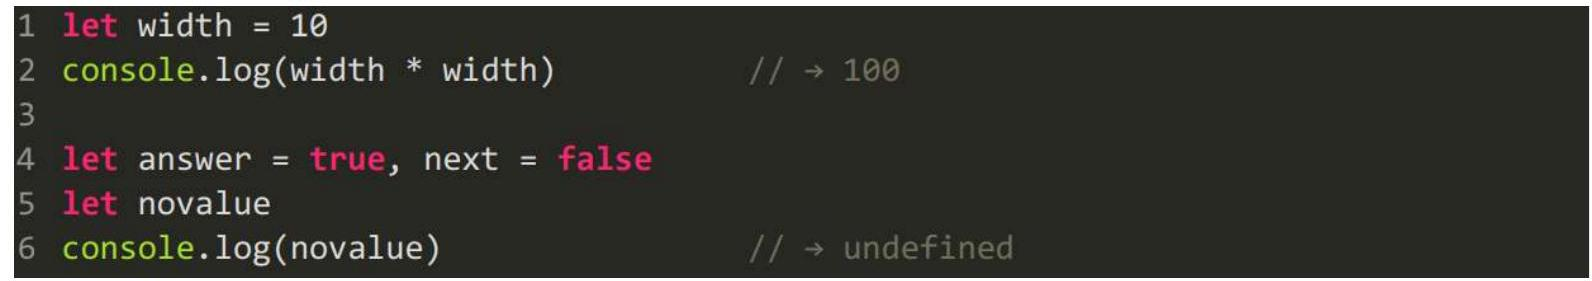
\includegraphics[width=\linewidth]{images/2024_12_29_858f09cde51177c71657g-05}
\end{center}

Var und const als keywords funktionieren auch.

\begin{verbatim}
switch (<ausdruck>) {
    case <wert1>:
    break
    default:
        ...
        break
}
\end{verbatim}

\begin{verbatim}
if (<ausdruck>) \{
\} else \{
\end{verbatim}

\}

\begin{verbatim}
for (let i=1; i<50; i*=2) {
    console.log(i)
}
4 // -> 1, -> 2, -> 4, > 8, > 16, -> 32
\end{verbatim}

Funktionsdefinition

\begin{verbatim}
1 const square = function (x) {
    return x * x
}
4
5 console.log(square(12)) // -> 144
\end{verbatim}

\begin{verbatim}
1 const square1 $=(x) \Rightarrow$ \{return $x * x$ \}
2 const square2 $=x=x^{*} x$
\end{verbatim}

Objekte und Arrays

\begin{center}
\begin{tabular}{|l|l|l|}
\hline
Was & Objekt & Array \\
\hline
Art & Attribut-Wert-Paare & Sequenz von Werten \\
\hline
Literalnotation & werte $=\{$ a: 1, b: 2$\}$ & liste $=[1,2,3]$ \\
\hline
Ohne Inhalt & werte $=\{ \}$ & liste $=[]$ \\
\hline
Elementzugriff & werte["a" $]$ oder werte.a & liste[0] \\
\hline
\end{tabular}
\end{center}

\section*{Objekte}
\begin{itemize}
  \item Objekt Attribute sind dynamisch und können einfach erweitert werden:
  \item Objekt Attribute können auch einfach mit dem delete keyword entfernt werden.
  \item Mit in kann überprüft werden, ob ein Attribut existiert
\end{itemize}

\begin{verbatim}
let person = {
    name: "John Baker",
    age: 23,
    "exam results": [5.5, 5.0, 5.0, 6.0, 4.5]
}
\end{verbatim}

\begin{verbatim}
    let obj = { message: "not yet implemented" }
    obj.ready = false
> obj
{ message: 'not yet implemented', ready: false }
> obj.attr
undefined
\end{verbatim}

\begin{verbatim}
> let obj = { message: "ready", ready: true, tasks: 3 }
> delete obj.message
> obj.tasks = undefined
> obj
{ ready: true, tasks: undefined }
> "message" in obj
false
> "tasks" in obj
true
\end{verbatim}

\section*{Methoden}
Ein Objekt kann auch Methoden enthalten:

\begin{verbatim}
> let cat = { type: "cat", sayHello: () => "Meow" }
> cat.sayHello
[Function: sayHello]
    > cat.sayHello()
'Meow'
\end{verbatim}

Arrays\\
Verschiedene Hilfsfunktionen:

\begin{itemize}
  \item Array.isArray()
  \item .push()
  \item .pop()
  \item Indexof, lastIndexOf
  \item Concat
  \item slice
  \item Shift, unshift
  \item .forEach(item => ....)
  \item .filter(item => .....)
  \item .map(item => ...)\\
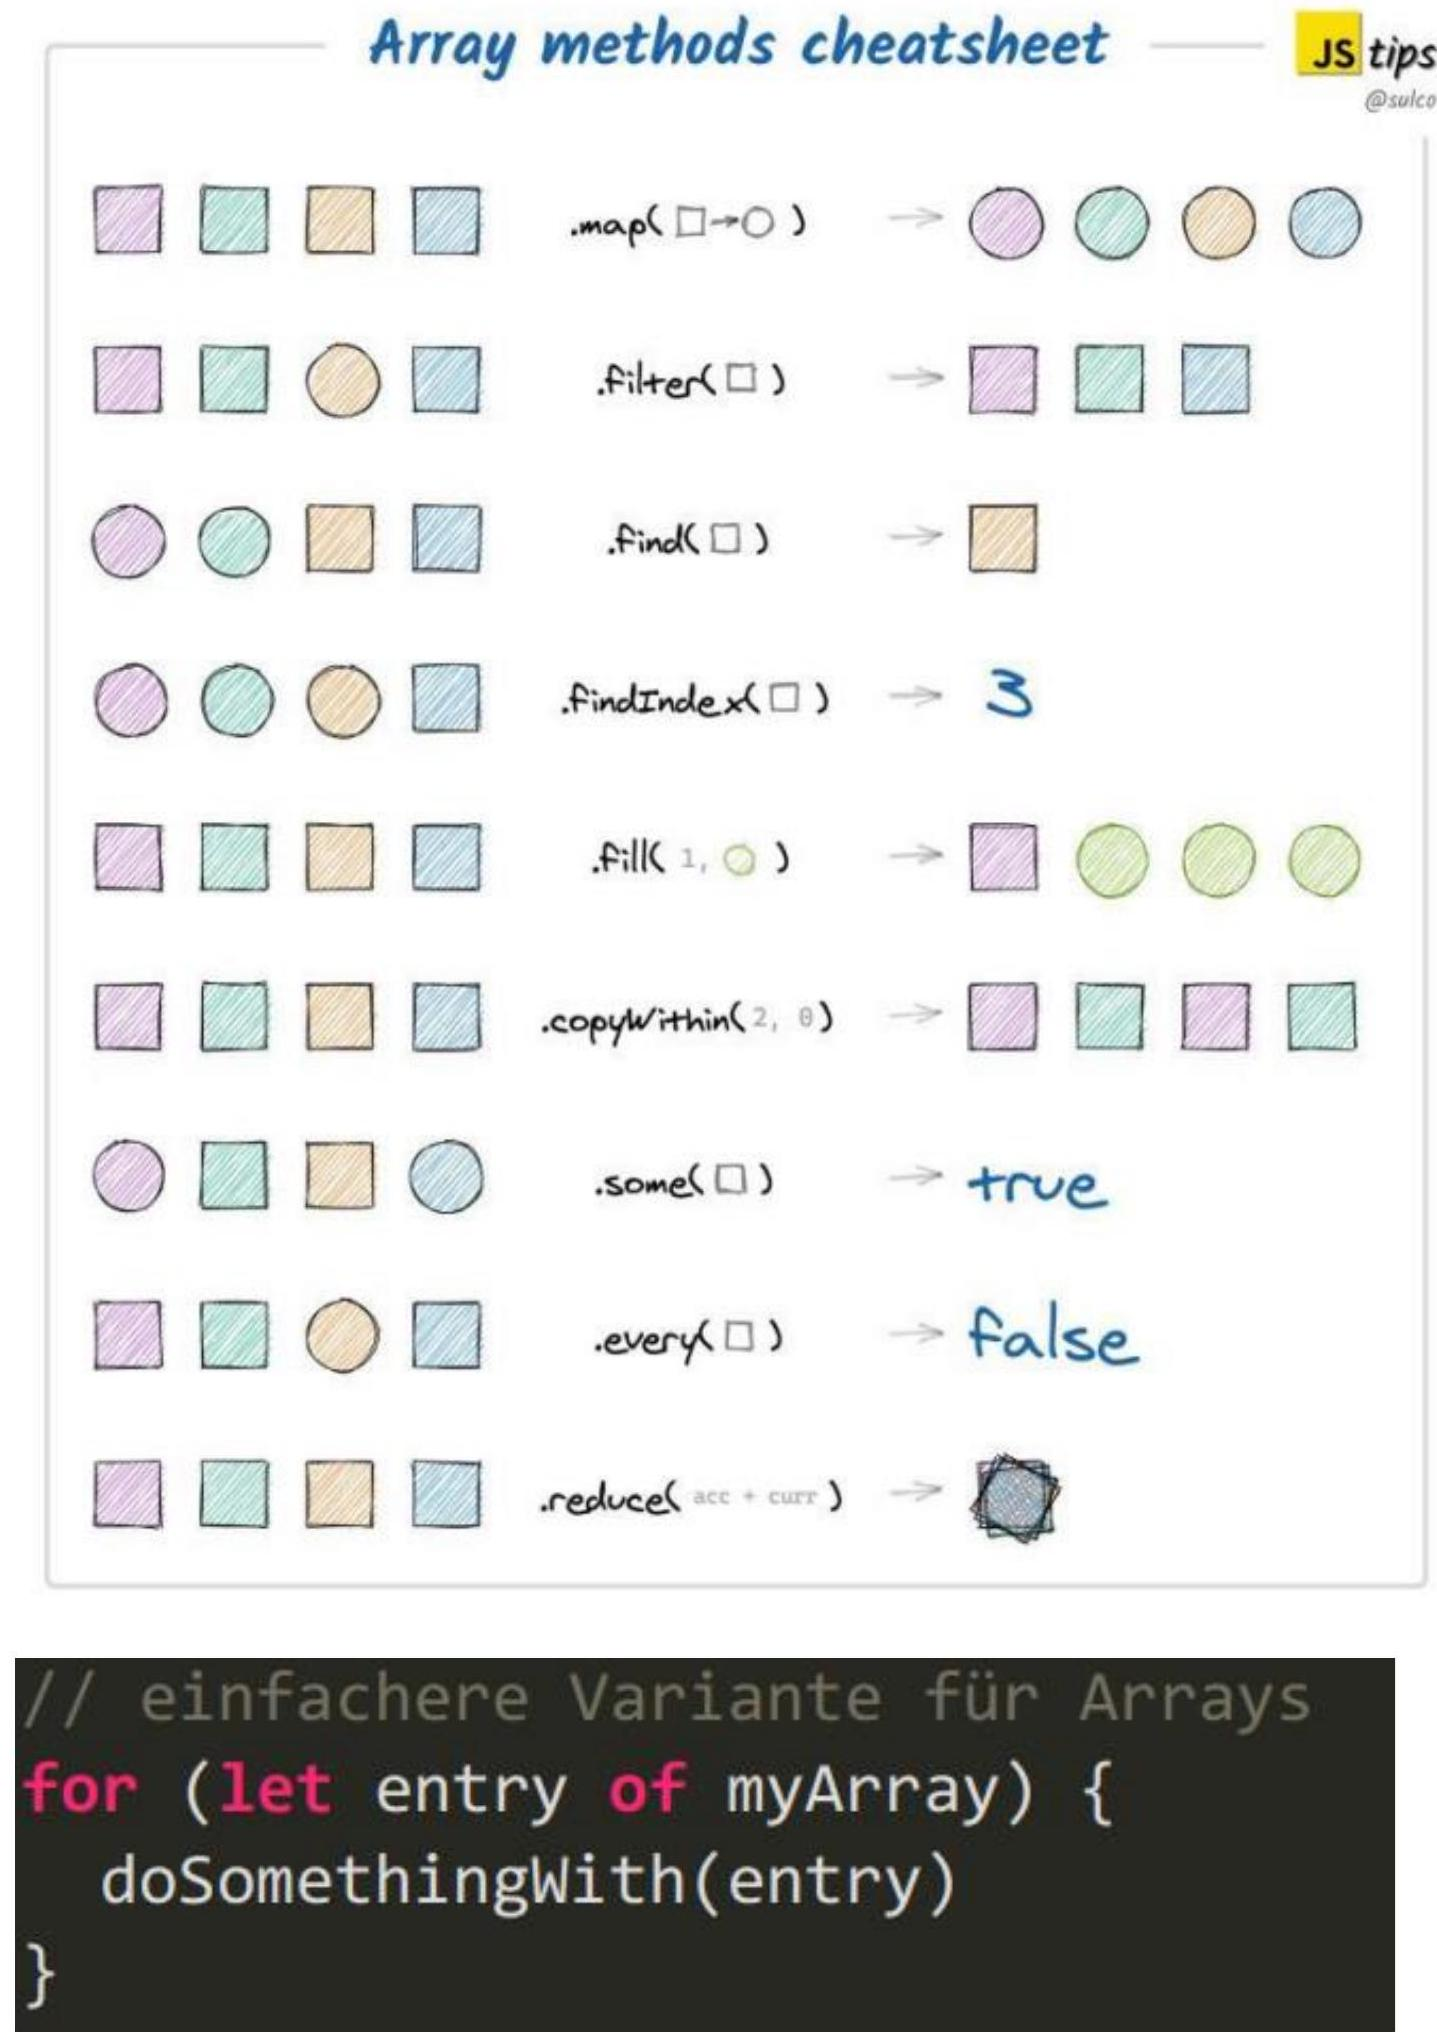
\includegraphics[width=\linewidth]{images/2024_12_29_858f09cde51177c71657g-08}
\end{itemize}

Json (JavaScript Object Notation)

\begin{itemize}
  \item Daten-Austauschformat, nicht nur für JavaScript
  \item Orientiert an Notation für JavaScript-Objektliterale
\end{itemize}

\begin{verbatim}
> JSON.stringify({ type: "cat", name: "Mimi", age: 3})
'{"type":"cat", "name":"Mimi", "age":3}'
> JSON.parse('{"type":"cat","name":"Mimi","age":3}')
{ type: 'cat', name: 'Mimi', age: 3 }
\end{verbatim}

\section*{https://www.json.org/json-en.html}
\section*{Funktionen}
\begin{itemize}
  \item Funktionen sind spezielle, aufrufbare Objekte
  \item Man kann ihnen jederzeit Attribute oder Methoden hinzufügen
  \item Sie haben bereits vordefinierte Methoden
\end{itemize}

\begin{verbatim}
const add = (x, y) => x + y
add.doc = "This function adds two values"
    add(3,4)
7
    add.doc
'This function adds two values'
\end{verbatim}

\section*{Modulsystem in JavaScript}
\begin{verbatim}
1 /* car-lib.js */
2}\mathrm{ const car = {
3 brand: 'Ford',
4 model: 'Fiesta'
5 }
6
7 module.exports = car
1 /* other js file */
2 const car = require('./car-lib')
\end{verbatim}

\section*{Prototypen von Objekten}
\begin{itemize}
  \item Die meisten Objekte haben ein Prototyp-Objekt.
  \item Dieses fungiert als Fallback für Attribute und Methoden.
\end{itemize}

\begin{verbatim}
> Object.getPrototypeOf(Math.max) == Function.prototype
true
> Object.getPrototypeOf([]) == Array.prototype
true
> Object.getPrototypeOf(Function.prototype) == Object.prototype
true
> Object.getPrototypeOf(Array.prototype) == Object.prototype
true
\end{verbatim}

\section*{PROTOTYPEN-KETTE}
\begin{verbatim}
function Employee (name, salary) {
    Person.call(this, name)
    this.salary = salary
}
Employee.prototype = new Person()
Employee.prototype.constructor = Employee
let e17 = new Employee("Mary", 7000)
console.log(e17.toString()) /* -> Person with name 'Mary' */
console.log(e17.salary) /* -> 7000 */
\end{verbatim}

Call, apply, bind

\begin{itemize}
  \item Weitere Argumente von call : Argumente der Funktion
  \item Weiteres Argument von apply : Array mit den Argumenten
  \item Erzeugt neue Funktion mit gebundenem this
\end{itemize}

\section*{Klassen}
\begin{verbatim}
class Person {
    constructor (name) {
        this.name = name
    }
    toString () {
        return `Person with name '${this.name}'
    }
}
let p35 = new Person("John")
console.log(p35.toString()) // -> Person with name 'John'
\end{verbatim}

\section*{Vererbung}
\begin{verbatim}
class Employee extends Person {
    constructor (name, salary) {
        super(name)
        this.salary = salary
    }
    toString () {
        return `${super.toString()} and salary ${this.salary}
    }
}
let e17 = new Employee("Mary", 7000);
console.log(e17.toString()) /* -> Person with name 'Mary' and salary 7000 */
console.log(e17.salary) /* -> 7000 */
\end{verbatim}

Getter und Setter

\begin{verbatim}
class PartTimeEmployee extends Employee {
    constructor (name, salary, percentage) {
        super(name, salary)
        this.percentage = percentage
    }
    get salary100 () { return this.salary * 100 / this.percentage}
    set salary100 (amount) { this.salary = amount * this.percentage / 100 }
}
let e18 = new PartTimeEmployee("Bob", 4000, 50)
console.log(e18.salary100) /* -> 8000 */
e18.salary100 = 9000
console.log(e18.salary) /* \ 4500 */
\end{verbatim}

Asynchrones Programmieren\\
File API\\
Mit require('fs') wird auf die File-Api zugegriffen.

\section*{Datei-Informationen}
\begin{verbatim}
const fs = require('fs')
fs.stat('test.txt' , (err, stats) => {
    if (err) {
    console.error(err)
    return
    }
    stats.isFile() /* true */
    stats.isDirectory() /* false */
    stats.isSymbolicLink() /* false */
stats.size /* 1024000 = ca 1MB */
})
\end{verbatim}

\section*{Pfade der Datei}
Um Pfad-informationen einer Datei zu ermitteln muss man dies mit require('path') machen.

\begin{verbatim}
const path = require('path')
const notes = '/users/bkrt/notes.txt'
path.dirname(notes) /* /users/bkrt */
path.basename(notes) /* notes.txt */
path.extname(notes) /* .txt */
path.basename(notes, path.extname(notes)) /* notes */
\end{verbatim}

\section*{Lesen aus einer Datei}
\begin{verbatim}
const fs = require('fs')
fs.readFile('/etc/hosts',"utf8", (err, data) => {
        if (err) throw err
        console.log(data)
})
\end{verbatim}

\section*{Dateien schreiben}
\begin{verbatim}
1 const fs = require('fs')
2}\mathrm{ const content = 'Node was here!'
3 fs.writeFile('/Users/bkrt/test.txt', content, (err) => {
4 if (err) {
5 console.error(`Failed to write file: ${err}`)
6 return
7 }
8 ** file written successfully */
9 })
\end{verbatim}

Weitere FS Funktionen

\begin{center}
\begin{tabular}{|l|l|}
\hline
Funktion & Bezeichnung \\
\hline
fs.access & Zugriff auf Datei oder Ordner prüfen \\
\hline
fs.mkdir & Verzeichnis anlegen \\
\hline
fs.readdir & Verzeichnis lesen, liefert Array von Einträgen \\
\hline
fs.rename & Verzeichnis umbenennen \\
\hline
fs.rmdir & Verzeichnis löschen \\
\hline
fs.chmod & Berechtigungen ändern \\
\hline
fs.chown & Besitzer und Gruppe ändern \\
\hline
fs.copyFile & Datei kopieren \\
\hline
fs.link & Besitzer und Gruppe ändern \\
\hline
fs.symlink & Symbolic Link anlegen \\
\hline
fs.watchFile & Datei auf Änderungen überwachen \\
\hline
\end{tabular}
\end{center}

\section*{Callbacks}
Ein Callback ist eine Funktion, welche als Argument einer anderen Funktion übergeben wird und erst aufgerufen wird, wenn das Ereignis eingetreten ist. In der folgenden Abbildung wird die KlickFunktion vom Button mit der Id «Button» abonniert.

1 document.getElementById('button').addEventListener('click', () => \{\\
2 //item clicked\\
3 \})

\section*{SetTimeout}
\begin{itemize}
  \item Mit setTimeout kann Code definiert werden, der zu einem späteren Zeitpunkt ausgeführt werden soll
  \item Eintrag in die Timer-Liste, auch wenn Zeit auf 0 gesetzt wird
  \item Kann mit clearTimeout entfernt werden
\end{itemize}

1 setTimeout(() => \{\\
2 /* runs after 50 milliseconds */\\
3 \}, 50)

\section*{SetInterval}
\begin{itemize}
  \item Callback alle n Millisekunden in die Callback Queue eingefügt
  \item Kann mit clearInterval beendet werden
\end{itemize}

\begin{verbatim}
1 const id = setInterval(() => {
2 // runs every 2 seconds
3 }, 2000)
4 clearInterval(id)
\end{verbatim}

\section*{SetImmediate}
\begin{verbatim}
1 setImmediate(() => {
2 console.log('immediate')
3 })
4
\end{verbatim}

\section*{Event-Modul (EventMitter)}
\begin{itemize}
  \item EventEmitter verwaltet Liste von Listeners zu bestimmten Events
  \item Listener für das Event können hinzugefügt oder entfernt werden
  \item Event kann ausgelöst werden $\rightarrow$ Listener werden informiert
\end{itemize}

\section*{Listener hinzufügen}
\begin{verbatim}
4 const EventEmitter = require('events')
5 const door = new EventEmitter()
6
7 door.on('open', () => \{
8 console.log('Door was opened')
9 \})
\end{verbatim}

\section*{Event auslösen}
\begin{verbatim}
1 door.on('open', (speed) => \{
2 console.log(`Door was opened, speed: \$\{speed /| 'unknown'\}`)
3 \})
4
5 door.emit('open')
6 door.emit('open', 'slow')
\end{verbatim}

\section*{Promises}
Ist ein Platzhalter für einen Wert, der erst später voraussichtlich verfügbar sein wird.

\begin{verbatim}
Funktion mit Promise
\end{verbatim}

\begin{verbatim}
function readFilePromise (file) {
\end{verbatim}

function readFilePromise (file) \{\\
let promise = new Promise(\\
let promise = new Promise(\\
function resolver (resolve, reject) \{\\
function resolver (resolve, reject) \{\\
fs.readFile(file, "utf8", (err, data) => \{\\
fs.readFile(file, "utf8", (err, data) => \{\\
if (err) reject(err)\\
if (err) reject(err)\\
else resolve(data)\\
else resolve(data)\\
\})\\
\})\\
\})\\
\})\\
return promise\\
return promise\\
\}

\begin{verbatim}
}
\end{verbatim}

Gibt nun ein Promise-Object zurück

\section*{Promise-Konstruktor erhlt resolver-Funktion}
Rückgabe einer Promise: potentieller Wert kann später erfüllt oder zurückgewiesen werden

\begin{itemize}
  \item Rückgabe einer Promise: potentieller Wert
  \item kann später erfüllt oder zurückgewiesen werden
\end{itemize}

Aufruf neu:

\begin{verbatim}
readFilePromise('/etc/hosts')
    .then(console.log)
    .catch(() => {
        console.log("Error reading file")
    })
\end{verbatim}

\section*{Promise-Zustände}
\begin{itemize}
  \item pending: Ausgangzustand
  \item fulfilled: erfolgreich abgeschlossen
  \item rejected: ohne Erfolg abgeschlossen
  \item Nur ein Zustandsübergang möglich
  \item Zustand in Promise-Objekt gekapselt\\
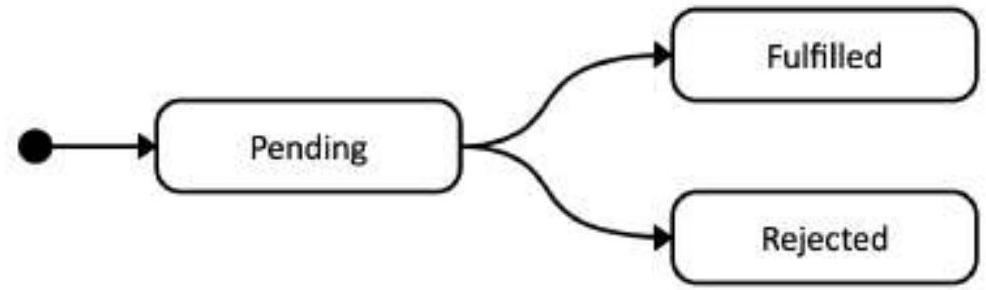
\includegraphics[width=\linewidth]{images/2024_12_29_858f09cde51177c71657g-14}
\end{itemize}

\section*{Promises Verknüpfen}
\begin{itemize}
  \item Then-Aufruf gibt selbst Promise zurück
  \item Catch-Aufruf ebenfalls, per Default erfüllt
  \item So können diese Aufrufe verkettet werden
  \item Promise, welche unmittelbar resolved wird: Promise.resolve (...)
  \item Promise, welche unmittelbar rejected wird: Promise.reject (...)
\end{itemize}

\section*{Promise.all()}
\begin{itemize}
  \item Erhält Array von Promises
  \item Erfüllt mit Array der Result, wenn alle erfüllt sind
  \item Zurückgewiesen sobald eine Promise zurückgewiesen wird
\end{itemize}

\section*{Promise.race()}
\begin{itemize}
  \item Erhält Array von Promises
  \item Erfüllt sobald eine davon erfüllt ist
  \item Zurückgewiesen sobald eine davon zurückgewiesen wird
\end{itemize}

\section*{ASYNC/AWAIT}
Beispiel 1

\begin{verbatim}
/* Bekanntes Beispiel */
const readHosts =() => {
    readFilePromise('/etc/hosts')
        .then(console.log)
        . catch(() => {
            console.log("Error reading file")
        })
}
/* Mit async/await */
const readHosts = async () => {
    try {
        console.log(await readFilePromise('/etc/hosts'))
    }
    catch (err) {
        console.log("Error reading file")
    }
}
\end{verbatim}

\section*{Beispiel 2}
\begin{verbatim}
function resolveAfter2Seconds (x) {
    return new Promise(resolve => {
        setTimeout(() => {
            resolve(x)
        }, 2000)
    })
}
async function add1(x) {
    var a = resolveAfter2Seconds(20)
    var b = resolveAfter2Seconds(30)
    return x + await a + await b
}
add1(10).then(console.log)
\end{verbatim}

\section*{Webserver}
Die Standard-Ports von einem Webserver sind 80 und 443. Der Webserver wartet auf eine Anfrage vom Client.

\section*{Server im Internet}
\begin{itemize}
  \item Wartet auf Anfragen auf bestimmtem Port
  \item Client stellt Verbindung her und sendet Anfrage
  \item Server beantwortet Anfrage
\end{itemize}

\begin{center}
\begin{tabular}{|l|l|}
\hline
Port & Service \\
\hline
$\mathbf{2 0}$ & FTP - Data \\
\hline
$\mathbf{2 1}$ & FTP - Control \\
\hline
$\mathbf{2 2}$ & SSH Remote Login Protocol \\
\hline
$\mathbf{2 3}$ & Telnet \\
\hline
$\mathbf{2 5}$ & Simple Mail Transfer Protocol (SMTP) \\
\hline
$\mathbf{5 3}$ & Domain Name System (DNS) \\
\hline
$\mathbf{8 0}$ & HTTP \\
\hline
$\mathbf{4 4 3}$ & HTTPs \\
\hline
\end{tabular}
\end{center}

File-Transfer (File Server)\\
Um Dateien auf einem File-Server auszutauschen, werden die Protokolle FTP (File Transfer Protocol) und SFTP (SSH File Transfer Protocol) verwendet.

HTTP\\
HTTP-Requests

\begin{center}
\begin{tabular}{|l|l|}
\hline
Methode & Beschreibung \\
\hline
GET & Ressource laden \\
\hline
POST & Information senden \\
\hline
PUT & Ressource anlegen, überschreiben \\
\hline
PATCH & Ressource anpassen \\
\hline
DELETE & Ressource löschen \\
\hline
\end{tabular}
\end{center}

HTTP-Response Codes

\begin{center}
\begin{tabular}{|l|l|}
\hline
Code & Beschreibung \\
\hline
$\mathbf{1 x x}$ & Information (101 Switching protocols) \\
\hline
$\mathbf{2 x x}$ & Erfolg (200 OK) \\
\hline
$\mathbf{3 x x}$ & Weiterleitung (301 Moved permanently) \\
\hline
$\mathbf{4 x x}$ & Fehler in Anfrage (403 Forbidden, 404 Not Found) \\
\hline
$\mathbf{5 x x}$ & Server-Fehler (501 Not implemented) \\
\hline
\end{tabular}
\end{center}

Node.js Webserver\\
Einfacher Webserver

\begin{verbatim}
const {createServer} = require("http")
Let server = createServer((request, response) => {
    response.writeHead(200, {"Content-Type": "text/html"})
    response.write(`
        <h1>Hello!</h1>
        <p>You asked for <code>${request.url}</code></p>`)
    response.end()
})
server.listen(8000)
console.log("Listening! (port 8000)")|
\end{verbatim}

\section*{Einfacher Webclient}
\begin{verbatim}
onst {request} = require("http")
let requestStream = request({
    hostname: "eloquentjavascript.net",
        path: "/20_node.html",
        method: "GET"
        headers: {Accept: "text/html"}
}, response => {
        console.log("Server responded with status code", response.statusCode)
})
requestStream.end()
\end{verbatim}

\section*{Server und Client mit Streams}
\begin{verbatim}
const {createServer} = require("http")
createServer((request, response) => {
    response.writeHead(200, {"Content-Type": "text/plain"})
        request.on("data", chunk =>
            response.write(chunk.toString().toUpperCase()))
        request.on("end" , () => response.end())
    }).listen(8000)
\end{verbatim}

\begin{verbatim}
const \{request\} = require("http")
Let $\mathrm{rq}=$ request(\{
    hostname: "localhost",
    port: 8000,
    method: "POST"
\}, response => \{
    response.on("data", chunk =>
    process.stdout.write(chunk.toString()));
\})
rq.write("Hello server\n")
rq.write("And good bye\n")
rq.end()
\end{verbatim}

\section*{REST API}
\begin{itemize}
  \item REST: Representational State Transfer
  \item Zugriff auf Ressourcen über ihre Adresse (URI)
  \item Kein Zustand: jede Anfrage komplett unabhängig
  \item Kein Bezug zu vorhergehenden Anfragen
  \item Alle nötigen Informationen in Anfrage enthalten
  \item Verwenden der HTTP-Methoden: GET , PUT , POST , ...\\
(WBE\_Alles.pdf) Page 363.\\
Express.js\\
Express.Js ist ein minimales, aber flexibles Framework für Web-apps. Es hat zahlreiche Utilities und Erweiterungen. Express.js basiert auf Node.js.
\end{itemize}

\section*{http://expressjs.com}
\section*{Installation}
\begin{itemize}
  \item Der Schritt npm init fragt eine Reihe von Informationen (Projektname, Version, ...) zum Projekt ab
  \item Als Entry Point ist hier index.js voreingestellt
  \item Das kann zum Beispiel in app.js geändert werden.
\end{itemize}

\begin{verbatim}
$ mkdir myapp
$ cd myapp
$ npm init
$ npm install express --save
\end{verbatim}

\section*{Beispiel: Express Server}
\begin{verbatim}
const express = require('express')
const app = express()
const port = 3000
app.get('/', (req, res) => {
        res.send('Hello World!')
})
app.listen(port, () => {
    console.log(`Example app listening at http://localhost:${port}`)
}})
\end{verbatim}

\begin{verbatim}
Routing
\end{verbatim}

\begin{verbatim}
app.get('/', function (req, res) {
\end{verbatim}

app.get('/', function (req, res) \{\\
res.send('Hello World!')\\
res.send('Hello World!')\\
\})\\
\})\\
app.post('/', function (req, res) \{\\
app.post('/', function (req, res) \{\\
res.send('Got a POST request')\\
res.send('Got a POST request')\\
\})\\
\})\\
app.put('/user', function (req, res) \{\\
app.put('/user', function (req, res) \{\\
res.send('Got a PUT request at /user')\\
res.send('Got a PUT request at /user')\\
\})\\
\})\\
app.delete('/user', function (req, res) \{\\
app.delete('/user', function (req, res) \{\\
res.send('Got a DELETE request at /user')\\
res.send('Got a DELETE request at /user')\\
\})

\begin{verbatim}
})
\end{verbatim}

Jasmine (Testing)

\section*{BEISPIEL (ZUGEHÖRIGE TESTS)}
\begin{verbatim}
/* PlayerSpec.js - Auszug */
describe("when song has been paused", function() {
    beforeEach(function() {
        player.play(song)
        player.pause()
    })
    it("should indicate that the song is currently paused", function() {
        expect(player.isPlaying).toBeFalsy()
        /* demonstrates use of 'not' with a custom matcher */
        expect(player).not.toBePlaying(song)
    })
    it("should be possible to resume", function() {
        player.resume()
        expect(player.isPlaying).toBeTruthy()
        expect(player.currentlyPlayingSong).toEqual(song)
    })
})
\end{verbatim}

\section*{JASMINE: MATCHER}
\begin{verbatim}
expect([1, 2, 3]).toEqual([1, 2, 3])
expect(12).toBeTruthy()
expect("").toBeFalsy()
expect("Hello planet").not.toContain("world")
expect(null).toBeNull()
expect(8).toBeGreaterThan(5)
expect(12.34).toBeCloseTo(12.3, 1)
expect("horse_ebooks.jpg").toMatch(/\w+.(jpg|gif|png|svg)/i)
\end{verbatim}

\section*{JASMINE: TESTS DURCHFÜHREN}
\$ npx jasmine\\
Randomized with seed 03741\\
Started

5 specs, 0 failures\\
Finished in 0.014 seconds\\
Randomized with seed 03741 (jasmine --random=true --seed=03741)

\section*{Browser-Technologien}
Vordefinierte Objekte

\begin{itemize}
  \item Die allgemeinen Objekte sind in JavaScript vordefiniert
  \item Tatsächlich handelt es sich um Funktionen/Konstruktoren
  \item Die Browser-Objekte existieren auf der Browser-Plattform
  \item Sie beziehen sich auf das Browser-Fenster, das angezeigte Dokument, oder den Browser selbst\\
document
  \item Repräsentiert die angezeigte Webseit
  \item Einstieg ins DOM (Document Object Model)
  \item Diverse Attribute und Methoden, zum Beispiel:
\end{itemize}

\begin{verbatim}
1 document.cookie /* Zugriff auf Cookies */
2 document.lastModified /* Zeit der letzten Änderung */
3 document.links /* die Verweise der Seite */
4 |document.images /* die Bilder der Seite */
\end{verbatim}

window

\begin{itemize}
  \item Repräsentiert das Browserfenster
  \item Zahlreiche Attribute und Methoden, u.a.:
  \item Alle globalen Variablen und Methoden sind hier angehängt
  \item Neue globale Variablen landen ebenfalls hier
\end{itemize}

\begin{verbatim}
1 window.document /* Zugriff auf Dokument */
2 window.history /* History-Objekt */
3 window.innerHeight /* Höhe des Viewports */
4 window.pageYOffset /* vertikal gescrollte Pixel */
5 window.alert === alert /* -> true */
6 window.setTimeout === setTimeout /* -> true */
7 window.parseInt === parseInt /* true */
\end{verbatim}

\section*{navigator}
Konsolen-eingabe auf dem folgenden Bild:

\begin{verbatim}
> navigator.userAgent
"Mozilla/5.0 (Macintosh; Intel Mac OS X 10.15; rv:91.0) Gecko/20100101 Firefox/91.0"
> navigator.language
"de"
> navigator.platform
"MacIntel"
> navigator.onLine
true
location
> location.href
"https://gburkert.github.io/selectors/"
> location.protocol
"https:"
> document.location.protocol
"https:"
\end{verbatim}

\section*{Document Object Model}
\begin{itemize}
  \item Element erzeugen: document.createElement
  \item Attribute erzeugen: document.createAttribute
  \item Und hinzufügen: .setAttribute
  \item Element in Baum einfügen: .appendChild
\end{itemize}

Element auffinden

\begin{verbatim}
1 let aboutus = document.getElementById("aboutus")
2 let aboutlinks = aboutus.getElementsByTagName("a")
3 let aboutimportant = aboutus.getElementsByClassName("important")
4 let navlinks = document.querySelectorAll("nav a")
\end{verbatim}

\section*{Textknoten erzeugen}
\begin{verbatim}
<p>The <img src="img/cat.png" alt="Cat"> in the
<img src="img/hat.png" alt="Hat">.</p>
<p><button onclick="replaceImages()">Replace</button></p>
<script>
    function replaceImages () {
        let images = document.body.getElementsByTagName("img")
        for (let i = images.length - 1; i >= 0; i--) {
                let image = images[i]
                if (image.alt) {
                let text = document.createTextNode(image.alt)
                image.parentNode.replaceChild(text, image)
                }
            }
    }
</script>
\end{verbatim}

Elementknoten erzeugen

\begin{verbatim}
<blockquote id="quote">
    No book can ever be finished. While working on it we learn ...
</blockquote>
<script>
/* definition of elt ... */
document.getElementById("quote").appendChild(
    elt("footer", "-",
    elt("strong", "Karl Popper"),
    ", preface to the second edition of ",
    elt("em", "The Open Society and Its Enemies"),
    ", 1950"))
</script>
\end{verbatim}

Attribut setzen\\
1

6

8

\begin{verbatim}
3 let att = document.createAttribute("class")
4 att.value ="democlass"
5 h1.setAttributeNode(att)
7 /* oder kürzer: */
let h1 = document.querySelector("h1")
,h1.setAttribute("class","democlass")
\end{verbatim}

Style anpassen\\
1 Nice text\\
2 

\section*{Event handling}
Event abonnieren/entfernen\\
Mit der Methode addEventListener() wird ein Event abonniert. Mit removeEventListener kann das Event entfernt werden.

\begin{verbatim}
<button>Act-once button</button>
<script>
    let button = document.querySelector("button")
    function once () {
        console.log("Done.")
        button.removeEventListener("click", once)
    }
    button.addEventListener("click", once)
</script>
\end{verbatim}

Wenn ein Parameter zur Methode hinzugefügt wird, wird dieses als das Event-Objekt gesetzt.

\begin{verbatim}
<script>
    let button = document.querySelector("button")
    button.addEventListener("click", (e) => {
        console.log("x="+e.x+", y="+e.y)
    })
</script\
\end{verbatim}

Das Event wird bei allen abonnierten Handlern ausgeführt bis ein Handler stopPropagation() ausführt.

\begin{verbatim}
<script>
    let button = document.querySelector("button")
    button.addEventListener("click", (e) => {
                console.log("x="+e.x+", y="+e.y)
                e.stopPropagation()
    })
</script>
\end{verbatim}

Viele Ereignisse haben ein Default verhalten. Eigene Handler werden vor Default-Verhalten ausgeführt. Um das Default-Verhalten zu verhindern, muss die Methode preventDefault() ausgeführt werden.

\begin{verbatim}
<a href="https://developer.mozilla.org/">MDN</a>
<script>
    let link = document.querySelector("a")
    link.addEventListener("click", event => {
            console.log("Nope.")
                event.preventDefault()
        })
,/script>
\end{verbatim}

\section*{Tastatur-Events}
\begin{itemize}
  \item keydown
  \item keyup
  \item Achtung: bei keydown kann das event mehrfach ausgelöst werden
\end{itemize}

\begin{verbatim}
<p>Press Control-Space to continue.</p>
<script>
    window.addEventListener("keydown", event => {
            if (event.key ==" " && event.ctrlKey) {
                console.log("Continuing!")
            }
    })
</script>
\end{verbatim}

Mauszeiger-Events

\begin{itemize}
  \item Mausklicks:
  \item mousedown
  \item mouseup
  \item click
  \item dblclick
  \item Mausbewegung
  \item mousemove
  \item Touch-display
  \item touchstart
  \item touchmove
  \item touched
\end{itemize}

\section*{Scroll-Events}
Das Scrollevent hat die Attribute des Event-Objekts: pageYOffset, pageXOffset.

\begin{verbatim}
window.addEventListener("scroll", () => {
    let max = document.body.scrollHeight - innerHeight
    bar.style.width = `${(pageYOffset / max) * 100}%`
,})
\end{verbatim}

Fokus- und Ladeereignisse

\begin{itemize}
  \item Fokus erhalten / verlieren
  \item focus
  \item blur
  \item Seite wurde geladen (ausgelöst auf window und document.body)
  \item load
  \item beforeunload
\end{itemize}

Jquery\\
JQuery ist eine freie JavaScript-Bibliothek, die Funktionen zur DOM-Navigation und -Manipulation zur Verfügung stellt.

\begin{verbatim}
$("button.continue").html("Next Step...")
var hiddenBox = $("#banner-message")
$("#button-container button").on("click", function(event) {
        hiddenBox.show()
    .})
\end{verbatim}

\begin{center}
\begin{tabular}{|c|c|c|}
\hline
Aufruf & Bedeutung & Beispiel \\
\hline
\$(Funktion) & DOM ready & \$(function0 \{ .... \}); \\
\hline
\multirow[t]{4}{*}{\$("CSS Selektor" ) .aktion(arg1, ....) .aktion(...)} & Wrapped Set & \$(".toggleButton").attr("title") \\
\hline
 & - Knoten, die Sel. erfüllen & \$(".toggleButton").attr("title", "click here") \\
\hline
 & - eingepackt in jQuery Obj. & \$(".toggleButton").attr((fitiel : "click here", ...)) \\
\hline
 &  & \texttt{\$(".toggleButton").attr("title", function0\{...\}) .css(...) .text(..) on("click", function(event) \{ ...\})} \\
\hline
\multirow[t]{2}{*}{\$("HTML-Code" )} & \begin{tabular}{l}
Wrapped Set \\
- neuer Knoten \\
\end{tabular} & \$("...").addClass(...) .appendTo("Selektor") \\
\hline
 & \begin{tabular}{l}
- eingepackt in jQuery Obj. \\
- noch nicht im DOM \\
\end{tabular} & \$("<li>>-.../li>").length \$("<li>...<li>")[0] \\
\hline
\multirow[t]{2}{*}{\$(DOM-Knoten)} & Wrapped Set & \$(document.body) \\
\hline
 & \begin{tabular}{l}
- dieser Knoten \\
- eingepackt in jQuery Obj. \\
\end{tabular} & \$(this) \\
\hline
\end{tabular}
\end{center}

\section*{Web-Grafiken}
\begin{itemize}
  \item Einfache Grafiken mit HTML und CSS möglich
  \item Zum Beispiel: Balkendiagramme
  \item Alternative für Vektorgrafiken: SVG
  \item Alternative für Pixelgrafiken: Canvas
\end{itemize}

SVG

\begin{itemize}
  \item Basiert wie HTML auf XML
  \item Elemente repräsentieren grafische Formen
  \item Ins DOM integriert und durch Scripts anpassbar
\end{itemize}

Beispiel:

\begin{verbatim}
p>Normal HTML here.</p>
<svg xmlns="http://www.w3.org/2000/svg">
    <circle r="50" cx="50" cy="50" fill="red"/>
    <rect x="120" y="5" width="90" height="90" stroke="blue" fill="none"/>
</svg>
\end{verbatim}

Ausgabe:\\
Normal HTML here.\\

\includegraphics[width=\linewidth]{images/2024_12_29_858f09cde51177c71657g-27}

JavaScript:

\begin{verbatim}
1 let circle = document.querySelector("circle")
2 circle.setAttribute("fill","cyan")
\end{verbatim}

\section*{Canvas}
\begin{itemize}
  \item Element canvas als Zeichenbereich im Dokument
  \item API zum Zeichnen auf dem Canvas
\end{itemize}

\begin{verbatim}
<canvas></canvas>
<script>
    Let cx = document.querySelector("canvas").getContext("2d")
    cx.beginPath()
    cx.moveTo(50, 10)
    cx.lineTo(10, 70)
    cx.lineTo(90, 70)
    cx.fill()
    let img = document.createElement("img")
    img.src = "img/hat.png"
    img.addEventListener("load" , () => {
        for (let x = 10; x < 200; x += 30) {
            cx.drawImage(img, x, 10)
        }
    })
</script>
\end{verbatim}

Canvas Methoden

\begin{center}
\begin{tabular}{|l|l|}
\hline
Methoden & Beschreibung \\
\hline
scale & Skalieren \\
\hline
translate & Koordinatensystem verschieben \\
\hline
rotate & Koordinatensystem rotieren \\
\hline
save & Transformationen auf Stack speichern \\
\hline
restore & Letzten Zustand wiederherstellen \\
\hline
\end{tabular}
\end{center}

Browser-API\\
Web Storage\\
Web Storage speichert Daten auf der Seite des Client.

\section*{Local Storage}
Local Storage wird verwendet, um Daten der Webseite lokal abzuspeichern. Die Daten bleiben nach dem Schliessen des Browsers erhalten. Die Daten sind in Developer Tools einsehbar und änderbar.

Die Daten werden nach Domains abgespeichert. Es können pro Webseite etwa 5MB abgespeichert werden.

\begin{verbatim}
1 localStorage.setItem("username","bkrt")
2 console.log(localStorage.getItem("username")) // -> bkrt
3 localStorage.removeItem("username")
\end{verbatim}

Die Werte werden als Strings gespeichert, daher müssen Objekte mit JSON codiert werden:\\
1 Let user = \{name: "Hans", highscore: 234\}\\
2 localStorage.setItem(JSON.stringify(user))

\section*{History}
History gibt zugriff auf den Verlauf des akutellen Fensters/Tab.

\begin{verbatim}
1 function goBack() {
2 window.history.back();
3
    ,}
\end{verbatim}

\begin{center}
\begin{tabular}{|l|l|}
\hline
Methoden & Beschreibung \\
\hline
length (Attribut) & \begin{tabular}{l}
Anzahl Einträgte inkl. aktueller Seite. Keine \\
Methode! \\
\end{tabular} \\
\hline
back & zurück zur letzten Seite \\
\hline
\end{tabular}
\end{center}

GeoLocation\\
Mit der GeoLocation-API kann der Standort abgefragt werden.

\begin{verbatim}
var options = { enableHighAccuracy: true, timeout: 5000, maximumAge: 0 }
function success(pos) {
    var crd = pos.coords
    console.log(`Latitude : ${crd.latitude}`)
    console.log(`Longitude: ${crd.longitude}`)
    console.log(`More or less ${crd.accuracy} meters.`)
}
function error(err) { ... }
navigator.geolocation.getCurrentPosition(success, error, options)
\end{verbatim}

\section*{Formulare}
Formulare ermöglichen Benutzereingaben. Sie gilt als Grundlade für Interaktion mit dem Web.\\
Input types:

\begin{itemize}
  \item submit, number, text, password, email, url , range , date , search , color
\end{itemize}

\begin{verbatim}
<form>
    <fieldset>
        <legend>General information</legend>
        <label>Text field <input type="text" value="hi"></label>
        <label>Password <input type="password" value="hi"></label>
        <label class="area">Textarea <textarea>hi</textarea></label>
    </fieldset>
    <fieldset>
        <legend>Additional information</legend>
        <label>Checkbox <input type="checkbox"></label>
        <label>Radio button <input type="radio" name="demo" checked></label>
        <label>Another one <input type="radio" name="demo"></label>
    </fieldset>
    <form>
    <label>Button <button>Click me</button></label>
    <label>Select menu
    <select name="cars">
    <option value="volvo">Volvo</option>
    <option value="saab">Saab</option>
    <option value="fiat">Fiat</option>
    <option value="audi">Audi</option>
    </select>
    </label>
    <input type="submit" value="Send">
</form>
|'
\end{verbatim}

\begin{center}
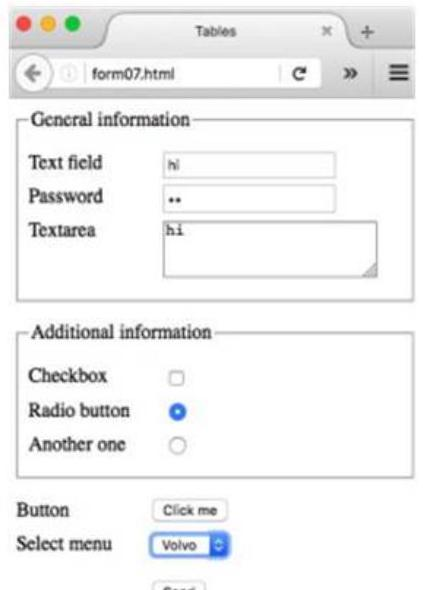
\includegraphics[width=\linewidth]{images/2024_12_29_858f09cde51177c71657g-29}
\end{center}

Formulare können auch POST/GET Aktionen ausführen:\\
Action beschreibt das Skript, welches die Daten annimmt. Method ist die Methode die ausgeführt wird.

\begin{verbatim}
<form action="/login" method="post">
2 ...
3 </form>
\end{verbatim}

\begin{center}
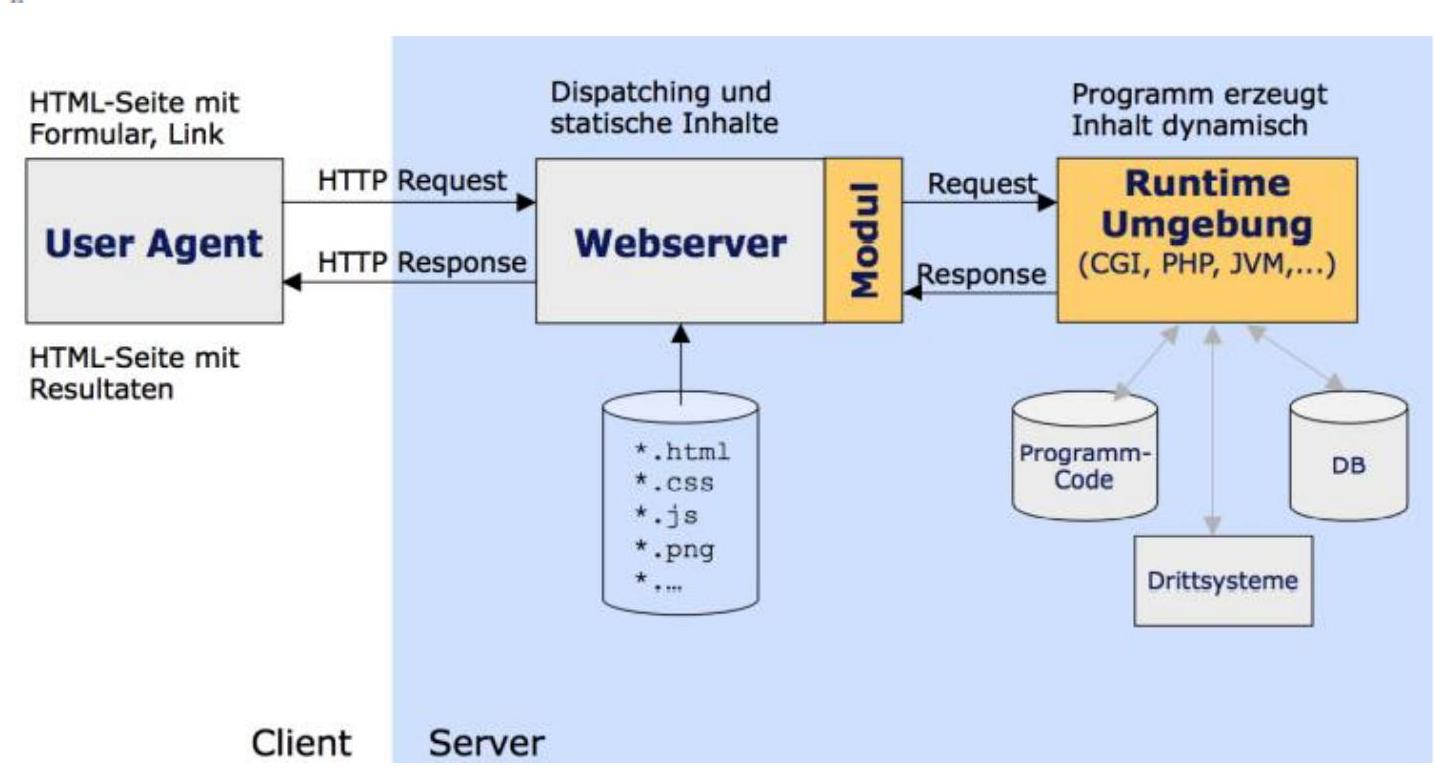
\includegraphics[width=\linewidth]{images/2024_12_29_858f09cde51177c71657g-29(1)}
\end{center}

Formular Events\\
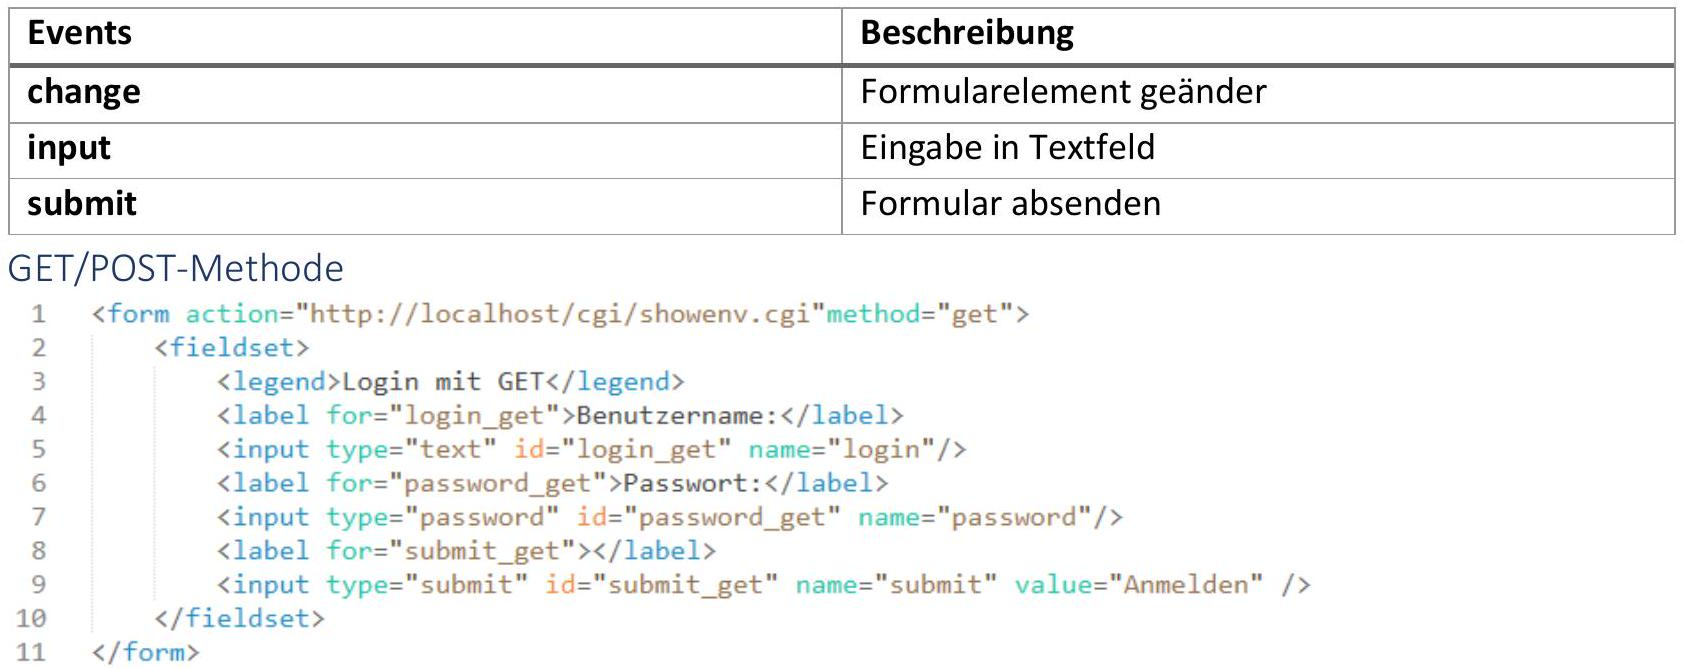
\includegraphics[width=\linewidth]{images/2024_12_29_858f09cde51177c71657g-30}

\section*{Cookies und Sessions}
Cookies

\begin{itemize}
  \item HTTP als zustandsloses Protokoll konzipiert
  \item Cookies: Speichern von Informationen auf dem Client
  \item Response: Set-Cookie -Header, Request: Cookie -Header
  \item Zugriff mit JavaScript möglich (ausser HttpOnly ist gesetzt)\\
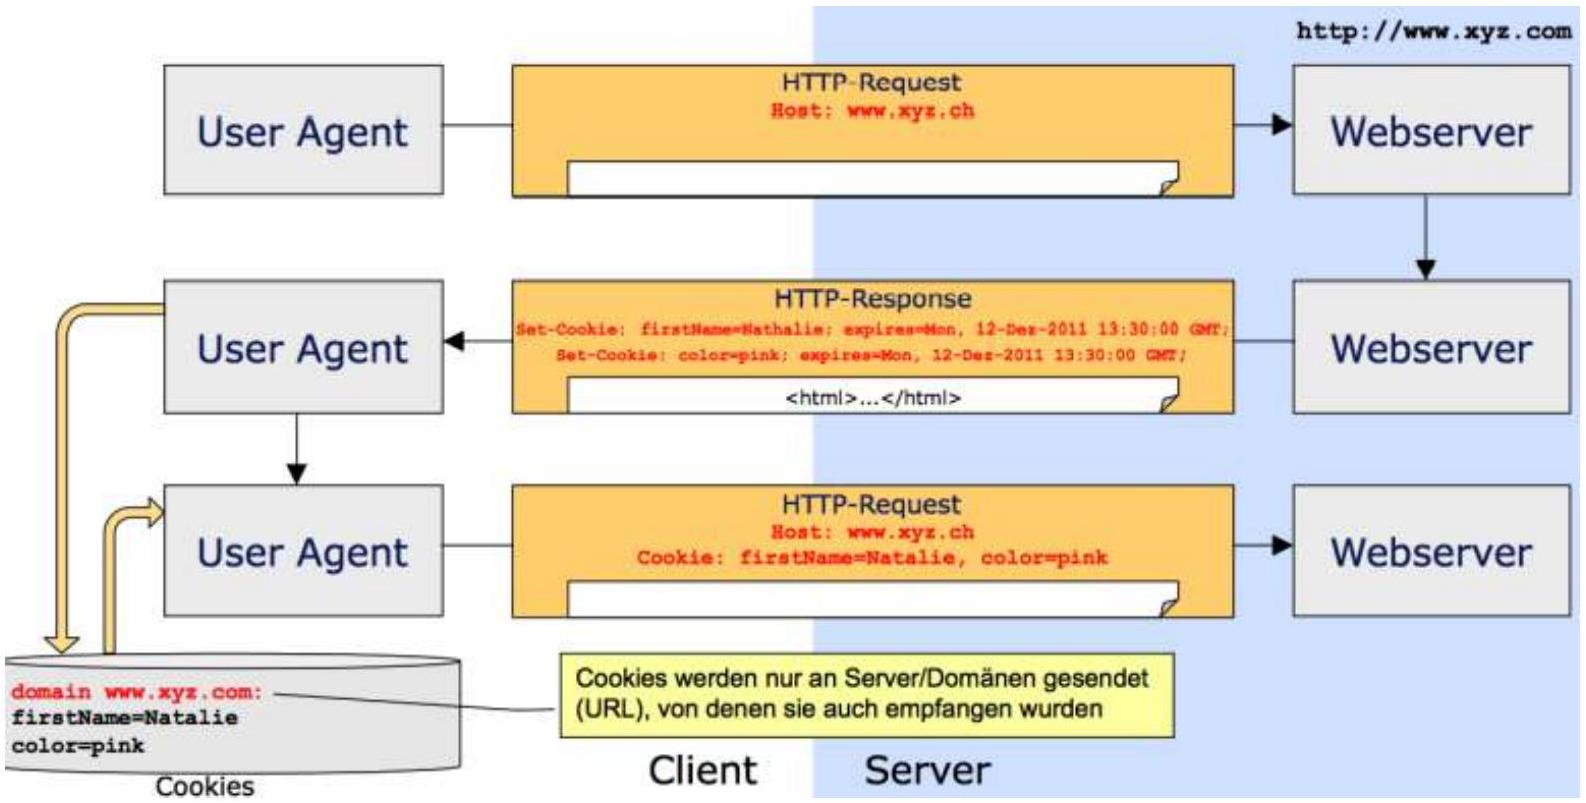
\includegraphics[width=\linewidth]{images/2024_12_29_858f09cde51177c71657g-31}
\end{itemize}

\section*{Sessions}
\begin{itemize}
  \item Cookies auf dem Client leicht manipulierbar
  \item Session: Client-spezifische Daten auf dem Server speichern
  \item Identifikation des Clients über Session-ID (Cookie o.a.)
  \item Gefahr: Session-ID gerät in falsche Hände (Session-Hijacking)
\end{itemize}

Ablauf:\\
\href{http://www.xyz.com}{http://www.xyz.com}\\
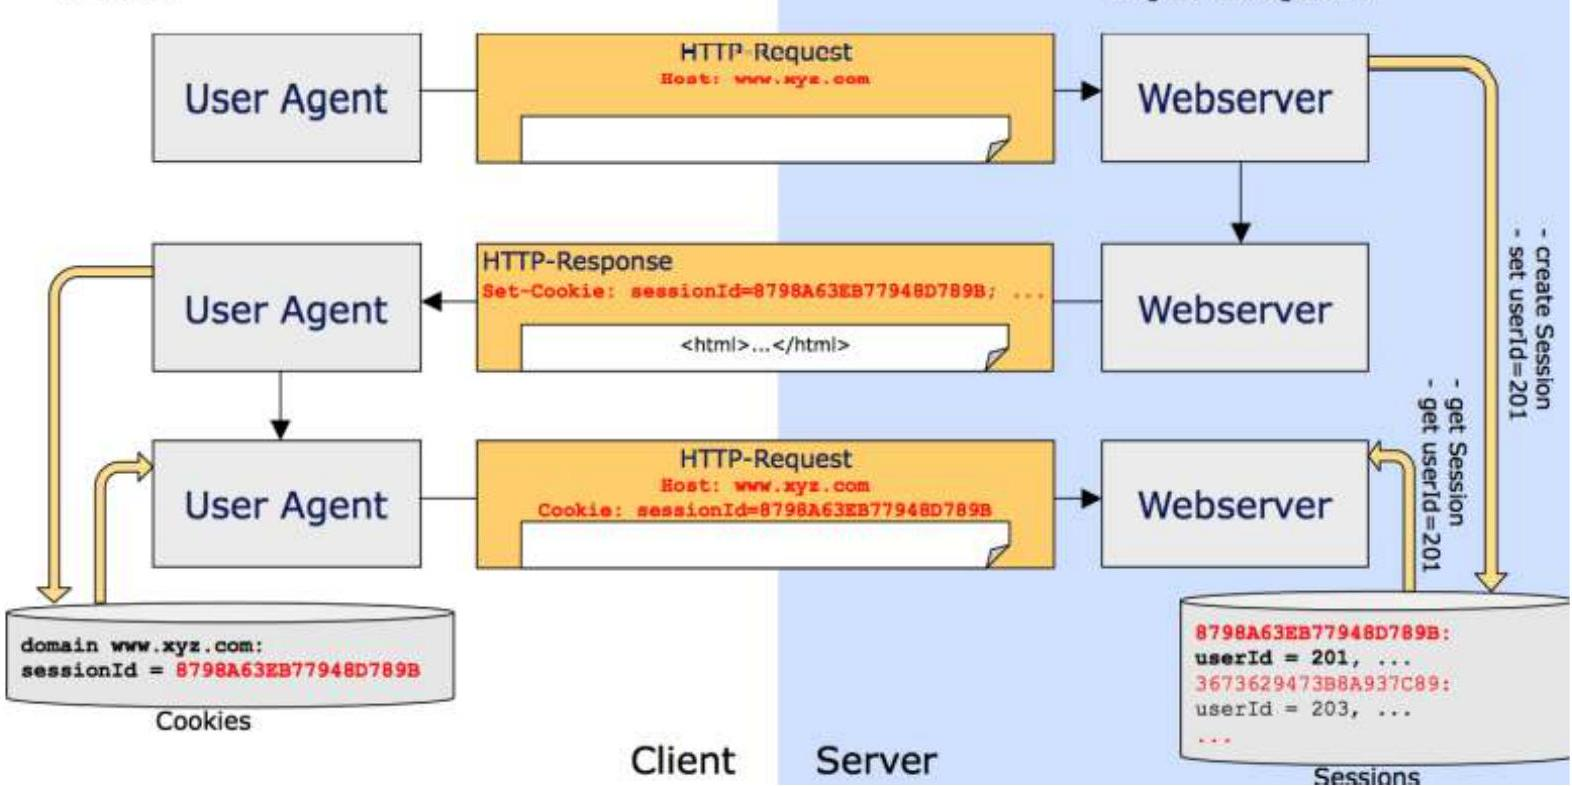
\includegraphics[width=\linewidth]{images/2024_12_29_858f09cde51177c71657g-31(1)}

\section*{Fetch API}
\begin{itemize}
  \item HTTP-Requests von JavaScripts
  \item Geben Promise zurück
  \item Nach Server-Antwort erfüllt mit Response-Objekt
\end{itemize}

\begin{verbatim}
fetch("example/data.txt")
.then(response => {
            console.log(response.status) // -> 200
    console.log(response.headers.get("Content-Type")) // -> text/plain
})
.then(resp => resp.text())
.then(text => console.log(text))
// -> This is the content of data.txt
\end{verbatim}

Response Objekt

\begin{itemize}
  \item headers : Zugriff auf HTTP-Header-Daten Methoden get, keys, forEach , ...
  \item status: Status-Code
  \item json() : liefert Promise mit Resultat der JSON-Verarbeitung
  \item text() : liefert Promise mit Inhalt der Server-Antwort
\end{itemize}

\section*{UI-Bibliothek}
Dom-Scripting und Abstraktionen\\
JSX und SJDON\\
SuiWeb


\end{document}